
\section{HAR en Android}
\begin{frame}{HAR en Android}

\framesubtitle{Arquitectura del Proyecto}

\setbeamercovered{transparent}
\begin{columns}

\column{0.5\textwidth}
\begin{itemize}
\item \textbf{HARDroid} 
\begin{itemize}
\item Es un servicio utilitario de reconocimiento.
\item Clasificador din�mico (\structure{DEX})
\end{itemize}

\pause{}
\item \textbf{ActivitySurvey}
\begin{itemize}
\item Aplicaci�n de encuesta que depende del servicio.
\item Registra evaluaciones de los usuarios. 
\end{itemize}

\pause{}
\item \textbf{Backend C4.5} 
\begin{itemize}
\item Servicio web de recolecci�n de evaluaciones.
\item Los aciertos son utilizados para mejorar el clasificador.
\end{itemize}
\end{itemize}

\column{0.5\textwidth}
\begin{center}
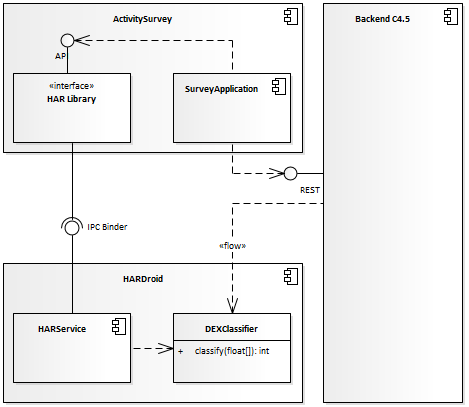
\includegraphics[width=1\columnwidth]{../capitulo-5/graphics/arqui_general}
\par\end{center}

\end{columns}

\end{frame}
%
\begin{frame}{HAR en Android}

\framesubtitle{Servicio de Reconocimiento}

\setbeamercovered{transparent}
\begin{columns}

\column{0.5\textwidth}
\begin{itemize}[<+->]
\item \structure{HARDroid} es un gestor en la capa de \emph{Application Framework}.
\item Mecanismo \structure{IPC} bajo el modelo \structure{Cliente-Servidor}.
\item Las aplicaciones m�viles hechas por terceros obtienen: 
\begin{itemize}
\item mejoras del motor de reconocimiento, 
\item actualizaci�n por plataforma de distribuci�n \structure{Google Play Store}, 
\item mecanismos f�ciles de integraci�n por \structure{Gradle}.
\end{itemize}
\end{itemize}

\column{0.5\textwidth}
\begin{overprint}
\onslide<1-2> 
\begin{center}
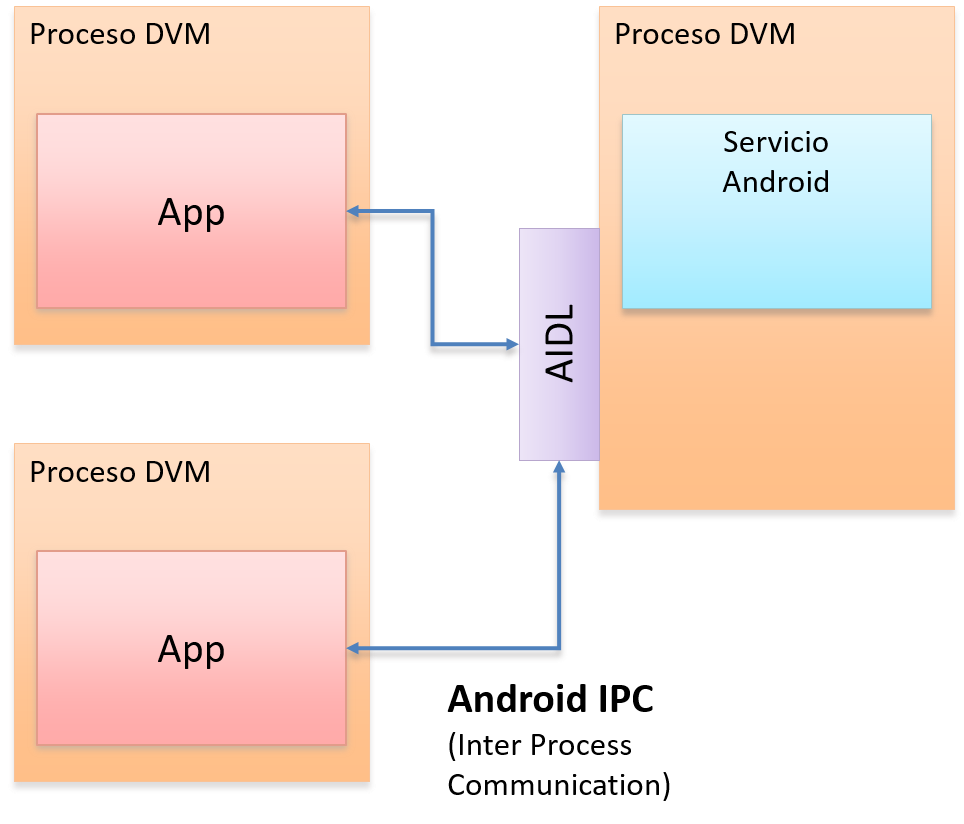
\includegraphics[width=1\columnwidth]{../capitulo-5/graphics/hardroid_func}
\par\end{center}
\onslide<3-> 
\begin{center}
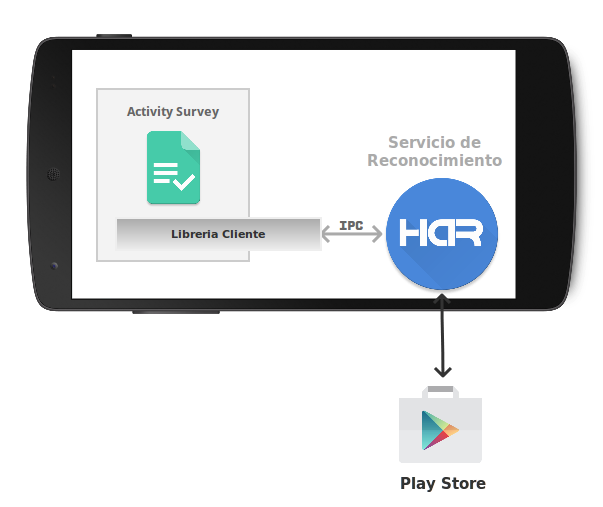
\includegraphics[width=1\columnwidth]{propuesta/graphics/archi_ipc}
\par\end{center}

\end{overprint}
\end{columns}

\end{frame}
%
\begin{frame}{HAR en Android}

\framesubtitle{HARDroid: M�dulos Funcionales}

\setbeamercovered{transparent}
\begin{columns}

\column{0.30\textwidth}
\begin{itemize}[<+->]
\item Integraci�n \structure{AIDL} 
\item Manejo de Sesi�n
\item Procesamiento de muestras
\item Reconocimiento de Actividades
\item Captura de se�ales
\end{itemize}
\begin{center}
\visible<5>{\begin{center}

\includegraphics[width=1.5cm]{propuesta/graphics/hardroid_logo}
\par\end{center}}
\par\end{center}

\column{0.70\textwidth}
\begin{center}
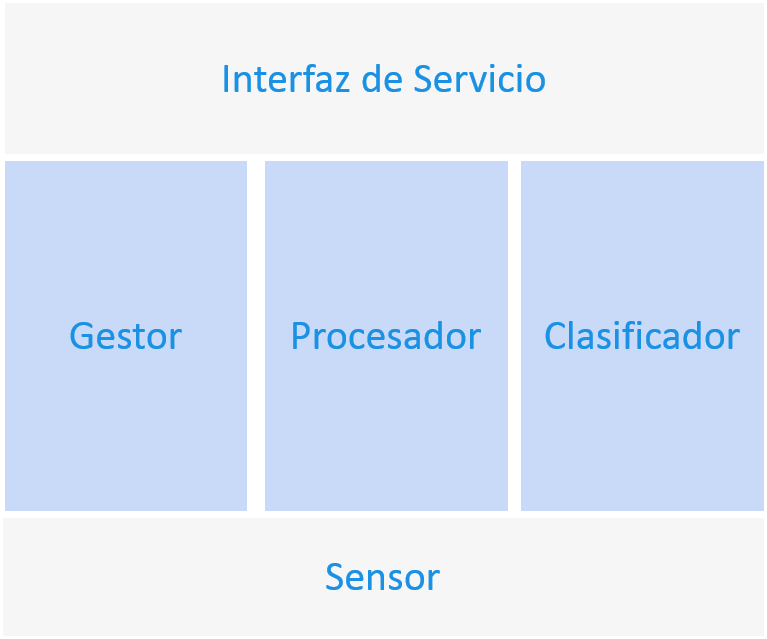
\includegraphics[width=0.9\columnwidth]{propuesta/graphics/hardroid}
\par\end{center}

\end{columns}

\end{frame}
%
\begin{frame}{HAR en Android}

\framesubtitle{Motor Reconocedor de Actividades}
\begin{center}
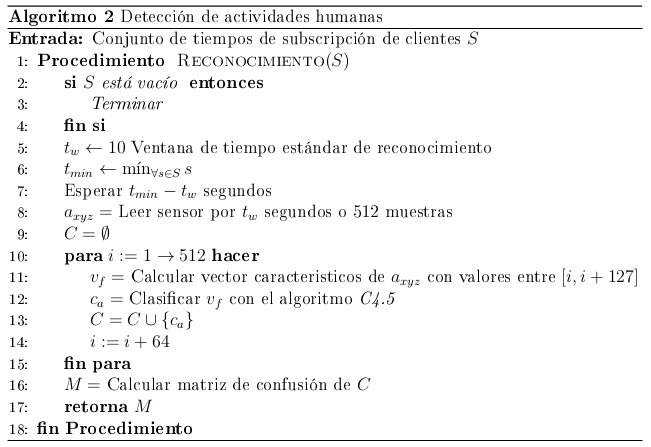
\includegraphics[width=0.8\columnwidth]{propuesta/graphics/algoritmoHAR}
\par\end{center}

\end{frame}
%
\begin{frame}{HAR en Android}

\framesubtitle{Activity Survey: M�dulos Funcionales}

\setbeamercovered{transparent}
\begin{columns}

\column{0.30\textwidth}
\begin{itemize}[<+->]
\item Presentaci�n
\item Identificaci�n
\item Encuesta guiada
\item Preferencias de comunicaci�n y notificaci�n
\item Almacenamiento y sincronizaci�n
\end{itemize}
\begin{center}
\visible<5>{\begin{center}

\includegraphics[width=1.5cm]{propuesta/graphics/activity_survey_logo}
\par\end{center}}
\par\end{center}

\column{0.70\textwidth}
\begin{center}
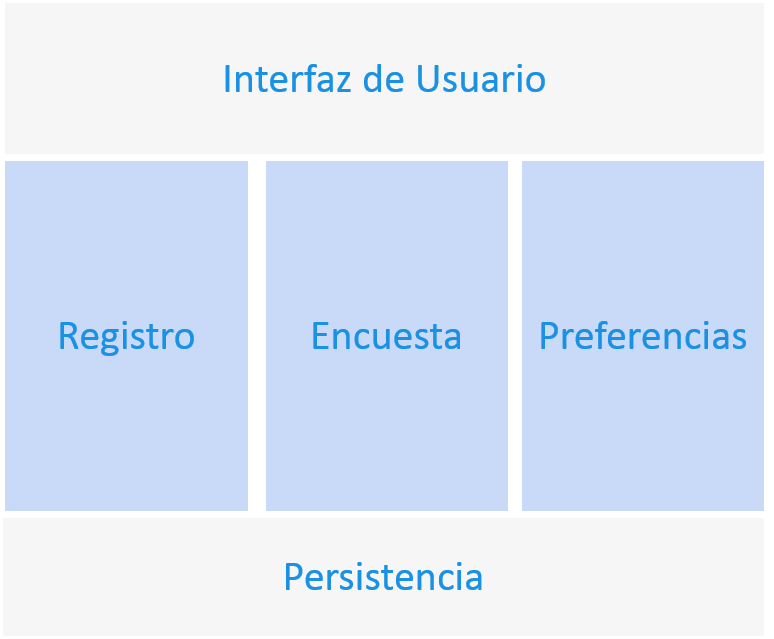
\includegraphics[width=0.9\columnwidth]{propuesta/graphics/activity_survey}
\par\end{center}

\end{columns}

\end{frame}
%
\begin{frame}{HAR en Android}

\framesubtitle{Activity Survey: Componentes Funcionales}
\begin{center}
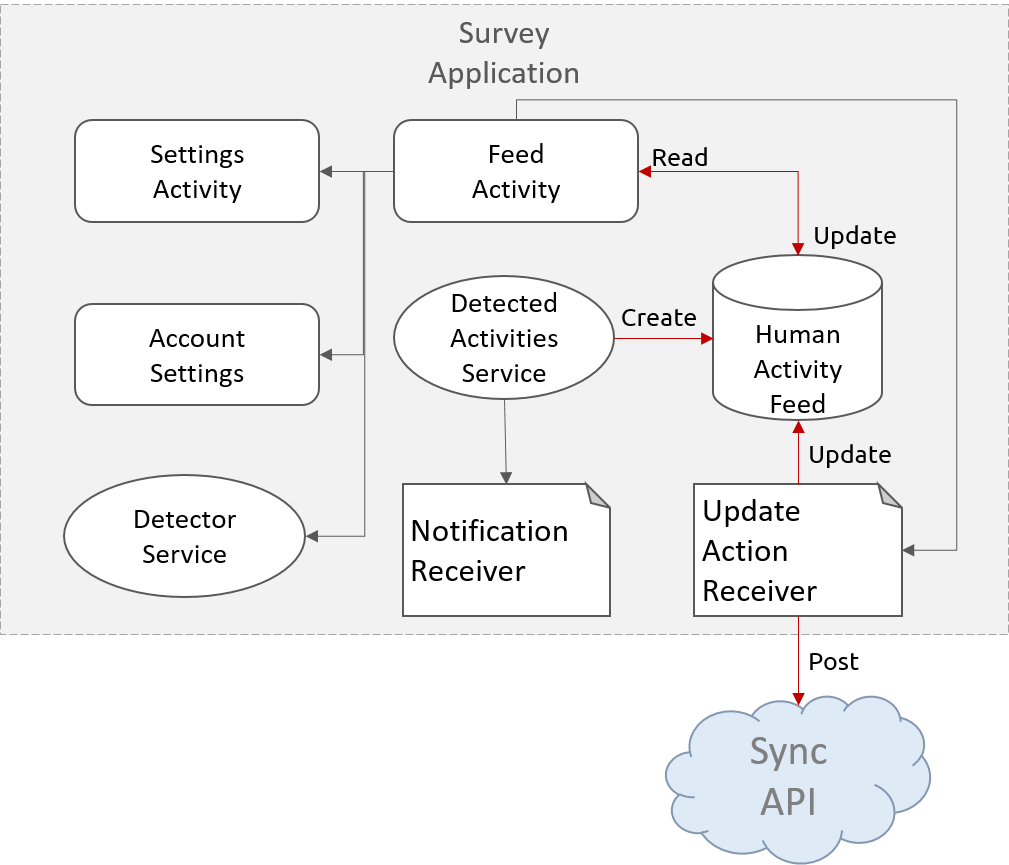
\includegraphics[width=0.65\columnwidth]{../capitulo-5/graphics/act_surv_diag}
\par\end{center}
\end{frame}

